\documentclass[12pt,a4paper]{article}

% ------------------------------------------------
% Pacotes
% ------------------------------------------------
\usepackage[utf8]{inputenc}
\usepackage[T1]{fontenc}
\usepackage[brazil]{babel}
\usepackage{graphicx}
\usepackage[table]{xcolor}
\usepackage{array}
\usepackage{tabularx}
\usepackage{geometry}
\usepackage{fancyhdr} 
\usepackage{mathptmx} % Times New Roman
\usepackage{enumitem}
\usepackage{amsfonts}
\usepackage{amsmath} % Recomendado para o comando \text{}
\usepackage{amssymb}
\usepackage{tikz}
\usetikzlibrary{positioning, shapes.geometric}

% TikZ Styles for ER Diagrams
\tikzset{
    block/.style={rectangle, draw, thick, minimum width=2cm, minimum height=1cm, fill=white},
    diamond_node/.style={diamond, draw, thick, minimum width=2cm, minimum height=1cm, fill=white, aspect=2},
    attribute/.style={ellipse, draw, thin, minimum width=1.5cm, minimum height=0.6cm, fill=white, font=\scriptsize},
    line/.style={draw, thick},
    specialization/.style={draw, circle, inner sep=1pt, font=\tiny, fill=white}
}
% ------------------------------------------------ 
% Configuração de página
% ------------------------------------------------
\geometry{
    a4paper,
    left=2cm,
    right=2cm,
    top=2cm,
    bottom=2cm,
    headheight=15pt
}
% Caixa para resposta discursiva
\newcommand{\resposta}[1]{
\noindent
\framebox[\textwidth]{
\begin{minipage}{0.98\textwidth}
\vspace{#1}
\end{minipage}
}
}

\pagestyle{fancy}
\fancyhf{}
\renewcommand{\headrulewidth}{0pt}

\setlength{\parindent}{0pt}

% ------------------------------------------------
% Comandos auxiliares
% ------------------------------------------------
\newcolumntype{L}[1]{>{\raggedright\arraybackslash}p{#1}}
\newcolumntype{C}[1]{>{\centering\arraybackslash}p{#1}}

% ------------------------------------------------
% Documento
% ------------------------------------------------
\begin{document}

% ------------------------------------------------
% Cabeçalho
% ------------------------------------------------
\begin{tabularx}{\textwidth}{@{} L{4cm} X @{}}
    \raisebox{-0.5cm}{
\includegraphics[width=4cm]{Universidade_de_Rio_Verde.jpg}} &
    \hfill
    \begin{tabular}{|>{\centering\arraybackslash}m{10cm}|>{\raggedright\arraybackslash}p{1.8cm}|}
        \hline
        \cellcolor{black}\color{white}\rule{0pt}{1.2cm}\textbf{ATIVIDADE DE REVISÃO} 
        & 
        \scriptsize Nota \tabularnewline
        \hline
    \end{tabular} 
\end{tabularx}
\vspace{0.3cm}


% ------------------------------------------------  
% Tabela principal - Estrutura limpa
% ------------------------------------------------
\begin{tabularx}{\textwidth}{|X|L{2cm}|}
\hline
\textbf{Curso} & \textbf{Campus} \\
\textit{Engenharia de Software} & \textit{Rio Verde} \\
\hline
\multicolumn{2}{|l|}{\textbf{Disciplina}} \\  
\multicolumn{2}{|l|}{ \textit{Banco de dados}} \\
\hline
\textbf{Nome do(a) acadêmico(a)} & \textbf{Valor} \\
& 7,0 \\
\hline
\textbf{Professor} & \textbf{Turma} \\
\textit{ Sergio Souza Novak} & \textit{B} \\
\hline
\textbf{Data da Avaliação} & \textbf{Código} \\
\textit{19/03/2026} & \textit{ESW417} \\
\hline
\end{tabularx}
 
% ------------------------------------------------
% Barra de Atenção
% ------------------------------------------------
\vspace{0.2cm}

\begin{tabularx}{\textwidth}{|X|}
\hline
\cellcolor{black}\color{white}
\centering \textbf{ATENÇÃO:} Somente serão passíveis de \textbf{REVISÃO} avaliações resolvidas à \textbf{TINTA}. \tabularnewline
\hline
\end{tabularx}

\vspace{0.3cm}

\textbf{ORIENTAÇÕES PARA A RESOLUÇÃO}  

\begin{itemize}
    \item A avaliação é individual, sem consulta;
    \item A interpretação de texto faz parte da avaliação;
\end{itemize}

\vspace{0.5cm}

\begin{center}
    \rule{\textwidth}{0.4pt}
    \textbf{QUESTÕES}
\end{center}

\vspace{0.5cm} 

\begin{enumerate}

      \item Considere a tabela \texttt{ContaBancaria} que armazena o identificador da conta, o nome do titular e o saldo atual. Qual comando SQL deve ser utilizado para selecionar \textbf{apenas} o nome do titular e o saldo de todas as contas cadastradas?

    \begin{enumerate}
        \item \texttt{SELECT * FROM ContaBancaria;}
        \item \texttt{SELECT titular, saldo FROM ContaBancaria;}
        \item \texttt{SELECT id\_conta, titular, saldo FROM ContaBancaria;}
        \item \texttt{GET titular, saldo FROM ContaBancaria;}
        \item \texttt{SELECT titular AND saldo FROM ContaBancaria;}
    \end{enumerate}


    \item Leia o texto e responda o que se pede, através de seus conhecimentos em banco de dados:
    
    
    A Páscoa de 2026 no Brasil se desenha em um contexto ambivalente, combinando sinais de otimismo do ponto de vista da indústria com maior cautela por parte dos consumidores diante do encarecimento dos chocolates. De um lado, entidades setoriais projetam uma data melhor do que a de 2025, apoiadas em cenário de inflação geral mais moderada, mercado de trabalho aquecido e expansão da oferta de produtos, inclusive com portfólios mais diversificados e número maior de itens presenteáveis nas gôndolas em relação ao ano anterior. De outro, os indicadores mostram que o chocolate segue acumulando alta de preços bastante acima da inflação média, o que pressiona o orçamento das famílias e leva muitos consumidores a pesquisar mais, migrar para marcas mais acessíveis ou substituir os tradicionais ovos por barras e produtos artesanais considerados financeiramente mais vantajosos.

Os dados recentes do IPCA apontam que, embora a inflação geral tenha desacelerado e a chamada “cesta de Páscoa” apresente variação menor em 2026 do que em 2025, o chocolate em barra, bombons e ovos ainda figuram entre os itens que mais encareceram no período, com aumentos próximos de 25% em doze meses. Nesse cenário, o setor produtivo mantém uma postura declaradamente otimista, apostando em aumento de produção, maior variedade de lançamentos e estratégias para manter acesso ao chocolate por meio de linhas mais econômicas, enquanto o consumidor adota uma postura mais seletiva, comparando preços, buscando promoções e, em muitos casos, recorrendo à produção caseira para reduzir custos. Assim, as notícias sobre a Páscoa de 2026 revelam menos um quadro de pessimismo generalizado e mais um ambiente de “otimismo cauteloso”: a indústria vislumbra crescimento nas vendas, mas esse avanço tende a se dar em meio à recomposição de preços e à necessidade de adaptação dos hábitos de consumo diante do encarecimento dos chocolates no país.

\noindent \textbf{Fonte:} \textit{ABICAB, Infomoney, Diário de Pernambuco, iG Economia, IPCA/IBGE e reportagens econômicas sobre o mercado de chocolates na Páscoa de 2026.}
    
    
    Uma fábrica de chocolates organiza sua produção de Páscoa registrando os ovos e suas respectivas linhas de produto de acordo com o Diagrama Entidade Relacionamento (DER) abaixo.

\begin{center}
\begin{tikzpicture}[node distance=2cm, every node/.style={scale=1}]
    % Entidades e Relacionamento
    \node[block] (ovo) {OVO};
    \node[diamond_node, right=of ovo] (pertence) {pertence};
    \node[block, right=of pertence] (tipo) {TIPO};
    
    % Atributos OVO
    \node[attribute, above=0.7cm of ovo] (id_o) {\underline{id\_ovo}};
    \node[attribute, below=0.7cm of ovo] (peso) {peso};
    \draw (ovo) -- (id_o);
    \draw (ovo) -- (peso);
    
    % Atributos TIPO
    \node[attribute, above=0.7cm of tipo] (id_t) {\underline{id\_tipo}};
    \node[attribute, below=0.7cm of tipo] (nome_t) {nome\_linha};
    \draw (tipo) -- (id_t);
    \draw (tipo) -- (nome_t);
    
    % Linhas e Cardinalidades
    \draw[line] (ovo) -- node[above] {(1,1)} (pertence);
    \draw[line] (pertence) -- node[above] {(0,n)} (tipo);
\end{tikzpicture}
\end{center}



A partir das regras de mapeamento do Modelo Conceitual para o Modelo Lógico Relacional, assinale a alternativa que apresenta o Esquema Relacional correto.

\begin{enumerate}[label=\Alph*)]
    \item \textbf{OVO}(\underline{id\_ovo}: inteiro, peso: real) \\
    \textbf{TIPO}(\underline{id\_tipo}: inteiro, nome\_linha: texto, id\_ovo: inteiro) \\
    \textit{id\_ovo referencia OVO(id\_ovo)}

    \item \textbf{OVO}(\underline{id\_ovo}: inteiro, peso: real, id\_tipo: inteiro) \\
    \textbf{TIPO}(\underline{id\_tipo}: inteiro, nome\_linha: texto) \\
    \textit{id\_tipo referencia TIPO(id\_tipo)}

    \item \textbf{PRODUCAO}(\underline{id\_ovo}: inteiro, peso: real, \underline{id\_tipo}: inteiro, nome\_linha: texto)

    \item \textbf{OVO}(\underline{id\_ovo}: inteiro, peso: real) \\
    \textbf{TIPO}(\underline{id\_tipo}: inteiro, nome\_linha: texto) \\
    \textit{(As tabelas não se conectam no modelo lógico)}

    \item \textbf{OVO}(\underline{id\_tipo}: inteiro, peso: real) \\
    \textbf{TIPO}(\underline{id\_ovo}: inteiro, nome\_linha: texto)
\end{enumerate}


\item Leia a tirinha e responda o que se pede: \\ 
\begin{center}
    % Substitua 'tirinha1' pelo nome do arquivo de imagem que você baixou
    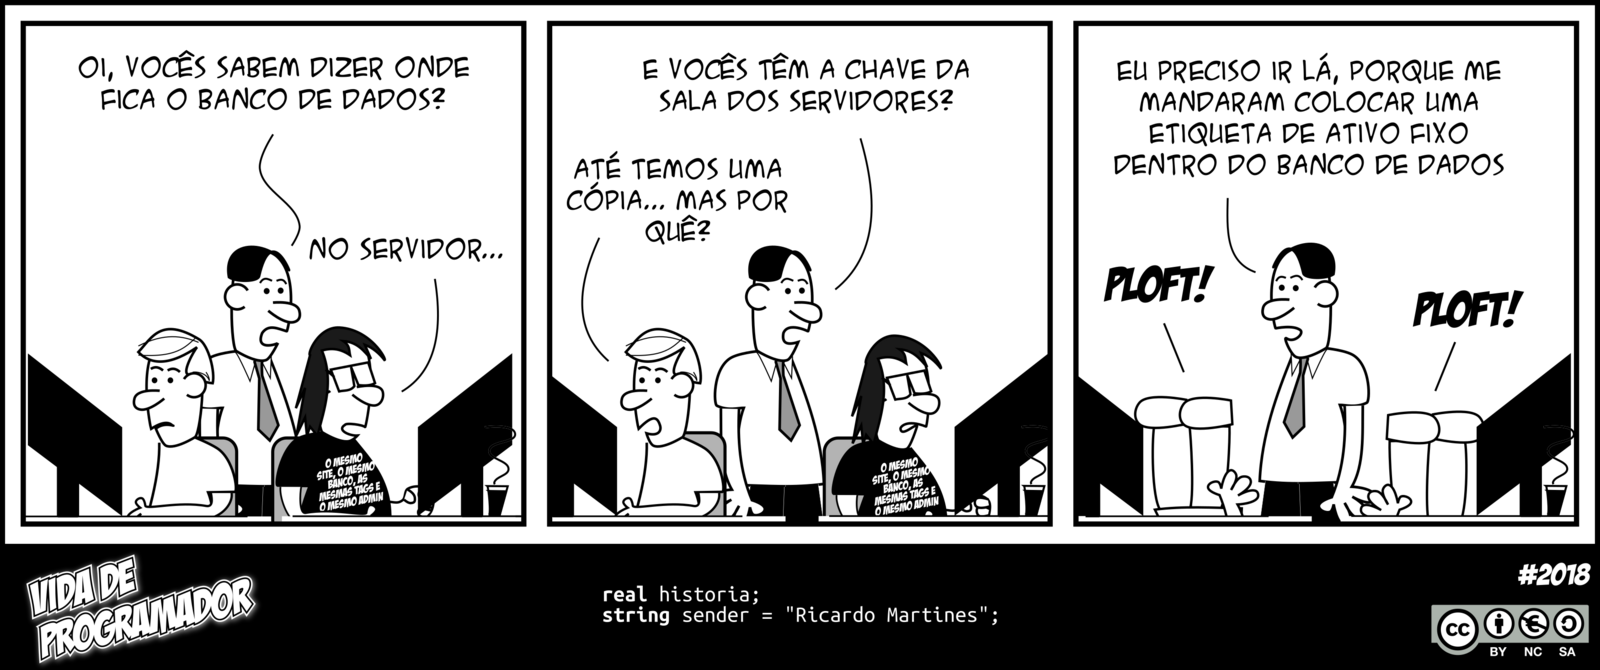
\includegraphics[width=0.85\textwidth]{tirinha2018.png} 
    
    \small \textbf{Tirinha 1:} \textit{Fonte: Vida de Programador. site: https://developerslife.tech/}
\end{center}

 
 
 
 No gerenciamento de infraestrutura de um Data Center, é necessário registrar a topologia da rede. O diagrama abaixo representa como um ativo de rede (como um Switch ou Roteador) pode estar conectado a outro ativo para fins de cascateamento ou redundância:

\begin{center}
\begin{tikzpicture}[node distance=2cm, every node/.style={scale=1}]
    % Entidade
    \node[block] (ativo) {ATIVO};
    
    % Atributos
    \node[attribute, left=1cm of ativo] (id) {\underline{id\_ativo}};
    \node[attribute, below left=0.7cm of ativo] (ip) {ip};
    \draw (ativo) -- (id);
    \draw (ativo) -- (ip);
    
    % Relacionamento (Auto-relacionamento)
    \node[diamond_node, above=1.5cm of ativo] (conecta) {conecta};
    
    % Linhas do Autorrelacionamento com cardinalidades
    % Linha que "sai" (lado N) e "volta" (lado 1)
    \draw[line] (ativo.east) -- ++(1.5,0) |- node[pos=0.25, right] {(0,n)} (conecta.east);
    \draw[line] (ativo.north) -- node[left] {(0,1)} (conecta.south);
    
\end{tikzpicture}
\end{center}



A partir das regras de mapeamento do Modelo Conceitual para o Modelo Lógico Relacional, assinale a alternativa que apresenta o Esquema Relacional mais adequado para este cenário.

\begin{enumerate}[label=\Alph*)]
    
    \item \textbf{ATIVO}(\underline{id\_ativo}: inteiro, ip: texto, id\_ativo\_superior: inteiro) \\
    \textit{id\_ativo\_superior referencia ATIVO(id\_ativo)}
    
    \item \textbf{ATIVO}(\underline{id\_ativo}: inteiro, ip: texto, id\_ativo: inteiro) \\
    \textit{id\_ativo referencia ATIVO(id\_ativo)}
    
    \item \textbf{ATIVO}(\underline{id\_ativo}: inteiro, ip: texto) \\
    \textbf{CONEXAO}(\underline{id\_ativo\_origem}: inteiro, \underline{id\_ativo\_destino}: inteiro)
    \item \textbf{ATIVO}(\underline{id\_ativo}: inteiro, ip: texto) \\
    \textit{(Autorrelacionamentos do tipo 1:N não são mapeados no modelo relacional)}

    \item \textbf{DATA\_CENTER}(\underline{id\_ativo}: inteiro, ip: texto, conexao: booleano)
\end{enumerate}
    \item A correta alocação da Chave Estrangeira (FK) é fundamental para evitar a redundância de dados e o excesso de valores nulos (NULL). Com base nas definições de mapeamento lógico e físico (SQL), responda o que se pede. Um Departamento possui Professores e Disciplinas. Um professor pode ministrar várias disciplinas, mas cada disciplina é ministrada por apenas um único professor. Assinale a alternativa correta em relação a onde a FK deve ser inserida:
    \begin{enumerate}[label=\Alph*)]
        \item A FK deve ser inserida na tabela \textbf{Professor}, pois é a entidade "forte".
        \item A FK deve ser inserida na tabela \textbf{Disciplina}, referenciando a Chave Primária de Professor.
        \item Deve-se criar uma terceira tabela para armazenar o relacionamento, por ser N:N.
        \item Ambos recebem FK um do outro para garantir a integridade.
        \item Não é necessário o uso de FK neste cenário.
    \end{enumerate}

    \item \textbf{Implementação SQL:} Com base no diagrama lógico abaixo, que representa a tabela \textbf{VEICULO} em um mapeamento de especialização/generalização (Tabela Única), escreva o código SQL (\texttt{CREATE TABLE}) para criar esta tabela. Utilize um campo \textbf{id} como Chave Primária (SERIAL) e garanta que o campo \textbf{chassi} seja único (UNIQUE). Apenas o campo \textbf{capacidade\_carga} pode ser nulo.

    \begin{center}
    \begin{tikzpicture}[node distance=0cm, outer sep=0pt, every node/.style={draw, rectangle, minimum height=0.7cm, font=\small, anchor=north west}]
        \node (header) [fill=gray!20, minimum width=11cm] at (0,0) {\textbf{Tab.: VEICULO}};
        
        \node (col1) [minimum width=2cm] at (0,-0.7cm) {id (PK)};
        \node (col2) [minimum width=3cm] at (2cm,-0.7cm) {chassi (UNIQUE)};
        \node (col3) [minimum width=3cm] at (5cm,-0.7cm) {modelo};
        \node (col4) [minimum width=3cm] at (8cm,-0.7cm) {capacidade\_carga};
        
        \node (r1c1) [minimum width=2cm] at (0,-1.4cm) {1};
        \node (r1c2) [minimum width=3cm] at (2cm,-1.4cm) {CH-111};
        \node (r1c3) [minimum width=3cm] at (5cm,-1.4cm) {Caminhão Volvo};
        \node (r1c4) [minimum width=3cm] at (8cm,-1.4cm) {30t};
        
        \node (r2c1) [minimum width=2cm] at (0,-2.1cm) {2};
        \node (r2c2) [minimum width=3cm] at (2cm,-2.1cm) {CH-222};
        \node (r2c3) [minimum width=3cm] at (5cm,-2.1cm) {Carro Fiat};
        \node (r2c4) [minimum width=3cm, fill=yellow!10] at (8cm,-2.1cm) {NULL};
    \end{tikzpicture}
    \end{center}

    \resposta{5.5cm}
\item Leia a tirinha e responda o que se pede: \\ 
\begin{center}
    % Substitua 'tirinha1' pelo nome do arquivo de imagem que você baixou
    \includegraphics[width=0.6\textwidth]{tirinha1} 
    
    \vspace{0.2cm}
    
    \small \textbf{Tirinha 2:} \textit{Fonte: Vida de Suporte. site: https://vidadesuporte.com.br/tag/banco-de-dados/}
\end{center}


Durante a manutenção de um banco de dados, um desenvolvedor precisa excluir a tabela \texttt{ContaBancaria}, mas deseja evitar que o sistema retorne um erro caso a tabela já tenha sido removida anteriormente. Qual comando SQL realiza essa operação de forma segura?

    \begin{enumerate}
        \item \texttt{DELETE TABLE ContaBancaria;}
        \item \texttt{DROP TABLE ContaBancaria IF EXISTS;}
        \item \texttt{REMOVE TABLE IF EXISTS ContaBancaria;}
        \item \texttt{DROP TABLE IF EXISTS ContaBancaria;}
        \item \texttt{CLEAR TABLE ContaBancaria;}
    \end{enumerate}



    \item Um Cliente pode comprar vários Produtos, e um produto pode ser comprado por vários clientes em diferentes instantes de tempo. Como este relacionamento é comumente resolvido no modelo lógico?
    \begin{enumerate}[label=\Alph*]
        \item Inserindo a FK de Cliente na tabela \textbf{Produto}.
        \item Inserindo a FK de Produto na tabela \textbf{Cliente}.
        \item Criando uma tabela associativa (ex: \textbf{Compra} ou \textbf{Venda}) que contém as FKs de ambas as tabelas originais.
        \item Mesclando as tabelas Cliente e Produto em uma só para consolidar dados de vendas.
        \item Transformando uma das entidades em um atributo multivalorado da outra.
    \end{enumerate}

 \item Com base no comando de criação de tabela abaixo, assinale a alternativa que apresenta o comando SQL (\texttt{INSERT INTO}) \textbf{correto} para inserir um novo registro na tabela \textbf{arvores}.

\begin{verbatim}
CREATE TABLE arvores (
    id TEXT,
    especie TEXT,
    altura DOUBLE PRECISION,
    diametro DOUBLE PRECISION,
    volume DOUBLE PRECISION,
    classe INTEGER,
    localizacao_x DOUBLE PRECISION,
    localizacao_y DOUBLE PRECISION
);
\end{verbatim}

\begin{enumerate}[label=\Alph*)]
    \item \texttt{INSERT INTO arvores (id, especie, altura) VALUES ('A1', 'Eucalipto', 15.5);}
    \item \texttt{INSERT arvores (especie, altura) VALUES ('Mogno', 20.0);}
    \item \texttt{ADD TO arvores (especie, altura) VALUES ('Mogno', 20.0);}
    \item \texttt{INSERT INTO arvores VALUES ('A1', 'Eucalipto', 15.5);}
    \item \texttt{INSERT INTO arvores ('A1', 'Eucalipto', 15.5);}
\end{enumerate}

\item Leia a tirinha e responda o que se pede: \\ 
\begin{center}
    % Substitua 'tirinha1' pelo nome do arquivo de imagem que você baixou
    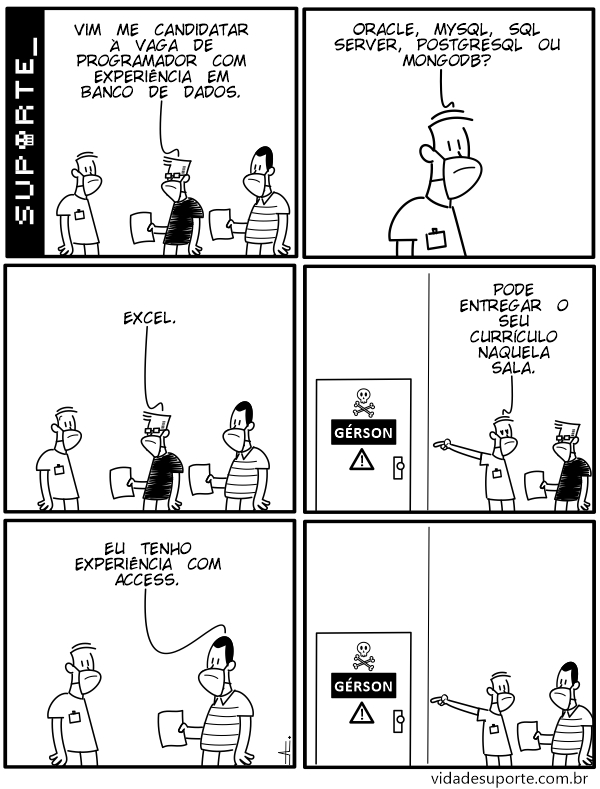
\includegraphics[width=0.6\textwidth]{Suporte_2781.jpg} 
    
    \small \textbf{Tirinha 3:} \textit{Fonte: Vida de Suporte. site: https://vidadesuporte.com.br/suporte-a-serie/experiencia-com-banco-de-dados/}
\end{center}

\noindent Na tirinha, \textbf{Oracle}, \textbf{MySQL}, \textbf{SQL Server}, \textbf{PostgreSQL} e \textbf{MongoDB} s{\~a}o exemplos de Sistemas de Gerenciamento de Banco de Dados (SGBDs). Essas ferramentas são profissionais, e são t{\'i}picas da {\'a}rea de desenvolvimento e administra{\c{c}}{\~a}o de bancos de dados, muito mais robustas que planilhas como \textit{Excel} ou bancos simples como \textit{Access}, por isso aparecem como crit{\'e}rio de ``experi{\^e}ncia s{\'e}ria'' na entrevista da tira. Sabendo disso, em suas palavras, crie um texto (de um parágrafo ou dois) explicando a diferença entre um Banco de dados e um Sistema de Gerenciamento de Banco de Dados.
\\

\resposta{6cm}

\vspace{0.8cm}


\item O sistema oficial da Copa do Mundo registra as participações de atletas e locais de jogo de acordo com o seguinte Diagrama Entidade Relacionamento (DER).

\begin{center}
\begin{tikzpicture}[node distance=1.5cm, every node/.style={scale=0.9}]
    % Entidades e Relacionamentos
    \node[block] (jogador) {JOGADOR};
    \node[diamond_node, right=of jogador] (atua) {atua};
    \node[block, right=of atua] (partida) {PARTIDA};
    \node[diamond_node, right=of partida] (ocorre) {ocorre};
    \node[block, right=of ocorre] (estadio) {ESTÁDIO};
    
    % Atributos JOGADOR
    \node[attribute, above=0.5cm of jogador] (pass) {\underline{id\_passaporte}};
    \node[attribute, below=0.5cm of jogador] (nome) {nome};
    \draw (jogador) -- (pass);
    \draw (jogador) -- (nome);
    
    % Atributos PARTIDA
    \node[attribute, above=0.5cm of partida] (cod_p) {\underline{cod\_partida}};
    \node[attribute, above right=0.5cm of partida] (data) {data};
    \node[attribute, below=0.5cm of partida] (fase) {fase};
    \draw (partida) -- (cod_p);
    \draw (partida) -- (data);
    \draw (partida) -- (fase);
    
    % Atributos ESTÁDIO
    \node[attribute, above=0.5cm of estadio] (cod_e) {\underline{id\_estadio}};
    \node[attribute, below=0.5cm of estadio] (nome_e) {nome\_estadio};
    \draw (estadio) -- (cod_e);
    \draw (estadio) -- (nome_e);
    
    % Linhas e Cardinalidades
    \draw[line] (jogador) -- node[above] {(0,n)} (atua);
    \draw[line] (atua) -- node[above] {(1,1)} (partida);
    
    \draw[line] (partida) -- node[above] {(1,1)} (ocorre);
    \draw[line] (ocorre) -- node[above] {(1,n)} (estadio);
\end{tikzpicture}
\end{center}

A partir das regras de mapeamento do Modelo Conceitual para o Modelo Lógico Relacional, assinale o Esquema Relacional mais adequado a ser gerado. Considere que as chaves primárias estão sublinhadas.

\begin{enumerate}[label=\Alph*]
    \item \textbf{PARTIDA}(\underline{cod\_partida}: inteiro, data: data, fase: texto) \\
    \textbf{JOGADOR}(\underline{id\_passaporte}: texto, nome: texto, cod\_partida: inteiro) \\
    \textit{cod\_partida referencia PARTIDA(cod\_partida)} \\
    \textbf{ESTÁDIO}(\underline{id\_estadio}: inteiro, nome\_estadio: texto, cod\_partida: inteiro) \\
    \textit{cod\_partida referencia PARTIDA(cod\_partida)}
    
    \item \textbf{JOGADOR}(\underline{id\_passaporte}: texto, nome: texto) \\
    \textbf{ESTÁDIO}(\underline{id\_estadio}: inteiro, nome\_estadio: texto) \\
    \textbf{PARTIDA}(\underline{cod\_partida}: inteiro, data: data, fase: texto, id\_estadio: inteiro, id\_passaporte: texto) \\
    \textit{id\_estadio referencia ESTÁDIO(id\_estadio)} \\
    \textit{id\_passaporte referencia JOGADOR(id\_passaporte)}
    
    \item \textbf{ESTÁDIO}(\underline{id\_estadio}: inteiro, nome\_estadio: texto) \\
    \textbf{PARTIDA}(\underline{cod\_partida}: inteiro, data: data, fase: texto, id\_estadio: inteiro) \\
    \textit{id\_estadio referencia ESTÁDIO(id\_estadio)} \\
    \textbf{JOGADOR}(\underline{id\_passaporte}: texto, nome: texto, cod\_partida: inteiro) \\
    \textit{cod\_partida referencia PARTIDA(cod\_partida)}
    
    \item \textbf{ESCALACAO\_GERAL}(\underline{cod\_partida}: inteiro, data: data, fase: texto, \underline{id\_passaporte}: texto, nome\_jogador: texto, id\_estadio: inteiro, nome\_estadio: texto)
    
    \item \textbf{JOGADOR}(\underline{id\_passaporte}: texto, nome: texto) \\
    \textbf{PARTIDA}(\underline{cod\_partida}: inteiro, data: data, fase: texto, id\_estadio: inteiro, nome\_estadio, id\_passaporte: texto) \\
    \textit{id\_passaporte referencia JOGADOR(id\_passaporte)}
\end{enumerate}  
\vspace{0.8cm}

 \item Um sistema de controle de chamados de tecnologia da informação registra os funcionários e os incidentes reportados na organização. A modelagem conceitual inicial produziu o diagrama entidade-relacionamento a seguir.

\begin{center}
\begin{tikzpicture}[node distance=2.5cm, every node/.style={scale=0.9}]
    \node[block] (funcionario) {FUNCIONARIO};
    \node[diamond_node, right=of funcionario] (relata) {relata};
    \node[block, right=of relata] (incidente) {INCIDENTE};
    
    \node[diamond_node, below=of incidente] (gera) {gera};
    \node[block, below=of gera] (notificacao) {NOTIFICACAO};
    
    \draw[line] (funcionario) -- node[above] {(0,n)} (relata);
    \draw[line] (relata) -- node[above] {(1,1)} (incidente);
    
    \draw[line] (incidente) -- node[right] {(0,n)} (gera);
    \draw[line] (gera) -- node[right] {(1,1)} (notificacao);
\end{tikzpicture}
\end{center}

A equipe de desenvolvimento deseja adicionar as seguintes características ao modelo:
\begin{enumerate}[label=\roman*]
    \item Cada notificação deve registrar as informações de data e horário exato de envio;
    \item As notificações devem ser enviadas apenas para a equipe (grupo de trabalho) do funcionário que relatou. Para isso, cada funcionário deve pertencer a um grupo (ex: grupo com vários membros da mesma área), e os membros desse grupo também devem usar a aplicação. Deseja-se armazenar quais notificações foram enviadas para quais funcionários específicos do grupo.
\end{enumerate}

Nessa situação, de forma análoga aos problemas clássicos de modelagem, adapte o diagrama ER da figura para atender aos novos requisitos. Desenhe as entidades, atributos e relacionamentos faltantes.

\vspace{0.2cm}
\resposta{16cm}

\vspace{0.8cm}

 \item Todo funcionário deve estar obrigatoriamente alocado a exatamente um departamento. Assinale a opção que representa corretamente, no modelo entidade-relacionamento, a especificação apresentada acima.

\begin{enumerate}[label=\Alph*]
    \item \begin{tikzpicture}[baseline=(rel.base), node distance=1.5cm, every node/.style={scale=0.8}]
        \node[block] (func) {funcionário};
        \node[diamond_node, right=of func] (rel) {alocação};
        \node[block, right=of rel] (depto) {departamento};
        \draw[line] (func) -- node[above] {(1,0)} node[below] {\scriptsize pertence a} (rel);
        \draw[line] (rel) -- node[above] {(n,0)} node[below] {\scriptsize possui} (depto);
    \end{tikzpicture}
    
    \item \begin{tikzpicture}[baseline=(rel.base), node distance=1.5cm, every node/.style={scale=0.8}]
        \node[block] (func) {funcionário};
        \node[diamond_node, right=of func] (rel) {alocação};
        \node[block, right=of rel] (depto) {departamento};
        \draw[line] (func) -- node[above] {(0,1)} node[below] {\scriptsize pertence a} (rel);
        \draw[line] (rel) -- node[above] {(0,n)} node[below] {\scriptsize possui} (depto);
    \end{tikzpicture}
    
    \item \begin{tikzpicture}[baseline=(rel.base), node distance=1.5cm, every node/.style={scale=0.8}]
        \node[block] (func) {funcionário};
        \node[diamond_node, right=of func] (rel) {alocação};
        \node[block, right=of rel] (depto) {departamento};
        \draw[line] (func) -- node[above] {(1,n)} node[below] {\scriptsize pertence a} (rel);
        \draw[line] (rel) -- node[above] {(0,n)} node[below] {\scriptsize possui} (depto);
    \end{tikzpicture}
     
    \item \begin{tikzpicture}[baseline=(rel.base), node distance=1.5cm, every node/.style={scale=0.8}]
        \node[block] (func) {funcionário};
        \node[diamond_node, right=of func] (rel) {alocação};
        \node[block, right=of rel] (depto) {departamento};
        \draw[line] (func) -- node[above] {(0,n)} node[below] {\scriptsize pertence a} (rel);
        \draw[line] (rel) -- node[above] {(0,n)} node[below] {\scriptsize possui} (depto);
    \end{tikzpicture}
    
    \item \begin{tikzpicture}[baseline=(rel.base), node distance=1.5cm, every node/.style={scale=0.8}]
        \node[block] (func) {funcionário};
        \node[diamond_node, right=of func] (rel) {alocação};
        \node[block, right=of rel] (depto) {departamento};
        \draw[line] (func) -- node[above] {(1,1)} node[below] {\scriptsize pertence a} (rel);
        \draw[line] (rel) -- node[above] {(0,n)} node[below] {\scriptsize possui} (depto);
    \end{tikzpicture}
\end{enumerate}

\vspace{0.8cm}

 \item O diagrama a seguir apresenta um relacionamento ternário entre \textbf{Médico}, \textbf{Paciente} e \textbf{Consultório}. Com base nas regras de conversão do modelo conceitual para o modelo lógico, realize a \textbf{eliminação do ternário}, transformando-o em um conjunto de relacionamentos binários ou utilizando uma entidade associativa de forma a manter a integridade das regras de negócio.

\begin{center}
\begin{tikzpicture}[node distance=2.5cm, every node/.style={scale=0.9}]
    % Entidades
     \node[block] (clinica) {Clínica};
    \node[block, below=of clinica] (consultorio) {Consultório};
    \node[block, left=of consultorio, xshift=-1cm] (paciente) {Paciente};
    \node[block, right=of consultorio, xshift=1cm] (medico) {Médico};

    
    \node[attribute, left=0.5cm of clinica] (cli_pk) {\underline{id\_cli}};
    \draw (clinica) -- (cli_pk);
    
    \node[attribute, right=0.5cm of consultorio] (cons_pk) {\underline{id\_cons}};
    \node[attribute, below right=0.5cm and 0.2cm of consultorio] (cons_sala) {sala};
    \draw (consultorio) -- (cons_pk);
    \draw (consultorio) -- (cons_sala);
    
    \node[attribute, above=0.5cm of paciente] (pac_pk) {\underline{cpf}};
    \node[attribute, above left=0.5cm and 0.5cm of paciente] (pac_nome) {nome};
    \draw (paciente) -- (pac_pk);
    \draw (paciente) -- (pac_nome);
    
    \node[attribute, above=0.5cm of medico] (med_pk) {\underline{id\_med}};
    \node[attribute, above right=0.5cm and 0.5cm of medico] (med_esp) {especialidade};
    \draw (medico) -- (med_pk);
    \draw (medico) -- (med_esp);
    
    % Relacionamentos Binários
    \node[diamond_node, below=1cm of clinica, yshift=0.5cm] (rel_local) {possui};
    
    % Relacionamento Ternário
    \node[diamond_node, below=1.5cm of consultorio] (rel_ternario) {consulta};
    \draw[line, <-] (rel_ternario) -- ++(3,-3) node[left] {Relacionamento Ternário}; % Apontando para o ternário
    
    % Linhas e Cardinalidades
    \draw[line] (clinica) -- node[right] {(1,1)} (rel_local);
    \draw[line] (rel_local) -- node[right] {(1,n)} (consultorio);
    
    % Conexões do Ternário
    \draw[line] (consultorio) -- node[left] {(1,n)} (rel_ternario);
    \draw[line] (paciente) |- node[near start, left, yshift=0.5cm] {(1,n)} (rel_ternario);
    \draw[line] (medico) |- node[near start, right, yshift=0.5cm] {(1,n)} (rel_ternario);
     
\end{tikzpicture}
\end{center}

\vspace{0.2cm}
\resposta{14cm}
\vspace{0.8cm}

 
\item Leia o texto introdutório e responda a questão a seguir:

\begin{center}
    \small \textbf{Estrutura de Cargos e Sal{\'a}rios da Universidade de Rio Verde (UniRV)}
\end{center}

\vspace{0.5cm}

A estrutura funcional da Universidade de Rio Verde (UniRV) organiza-se como um reflexo direto de sua natureza jur{\'i}dica de autarquia municipal. Nesse cen{\'a}rio, tanto a composi{\c{c}}{\~a}o dos cargos quanto a defini{\c{c}}{\~a}o dos sal{\'a}rios e as possibilidades de progress{\~a}o na carreira s{\~a}o regidas por um conjunto de leis municipais e detalhadas nos editais de seus concursos p{\'u}blicos, garantindo seguran{\c{c}}a jur{\'i}dica e transpar{\^e}ncia ao servidor.

O corpo de profissionais da institui{\c{c}}{\~a}o divide-se, essencialmente, entre o quadro docente e o t{\'e}cnico-administrativo. Para os professores, a carreira {\'e} moldada pela titula{\c{c}}{\~a}o, distinguindo-se entre especialistas, mestres e doutores, com regimes de trabalho que podem variar de 20 a 40 horas semanais. J{\'a} o setor administrativo abrange uma vasta gama de fun{\c{c}}{\~o}es que exigem desde o n{\'i}vel fundamental at{\'e} o superior, englobando postos que v{\~a}o de auxiliares de servi{\c{c}}os gerais a procuradores jur{\'i}dicos.

No que tange {\`a} remunera{\c{c}}{\~a}o, os valores s{\~a}o periodicamente ajustados por meio de reposi{\c{c}}{\~o}es salariais autorizadas pelo Legislativo local. Enquanto os professores podem ser remunerados por hora-aula --- com valores previstos em cerca de 52,62 reais para substitutos em 2026 --- ou por vencimentos fixos previstos no Plano de Carreira, os servidores administrativos encontram vencimentos que variam conforme a complexidade da fun{\c{c}}{\~a}o, com patamares que alcan{\c{c}}am aproximadamente 3.036,00 reais em editais recentes para cargos t{\'e}cnicos. Al{\'e}m do sal{\'a}rio base, a UniRV oferece mecanismos de valoriza{\c{c}}{\~a}o profissional, como gratifica{\c{c}}{\~o}es por produtividade e abonos, permitindo que o servidor ascenda na carreira conforme seu tempo de servi{\c{c}}o e o constante aprimoramento de suas qualifica{\c{c}}{\~o}es.


\noindent \textbf{Fonte:} \textit{Portal da Transpar{\^e}ncia da UniRV e Editais de Concursos P{\'u}blicos (vestibularunirv.com.br).}


No projeto do novo Banco de Dados de Recursos Humanos da \textbf{Universidade de Rio Verde (UniRV)}, a equipe de analistas utilizou o modelo abaixo para representar a hierarquia de cargos e a herança de propriedades entre os colaboradores:

\begin{center}
\begin{tikzpicture}[node distance=1.2cm, every node/.style={scale=0.9}]
    % NÍVEL 1: Superclasse Raiz
    \node[block] (servidor) {SERVIDOR\_UNIRV};
    \node[attribute, above=0.5cm of servidor] (mat) {\underline{matricula}};
    \node[attribute, right=0.3cm of mat] (nome) {nome};
    \draw (servidor) -- (mat); \draw (servidor) -- (nome);

    % Símbolo de Especialização 1
    \node[specialization, below=0.8cm of servidor] (spec1) {d};
    \draw[line] (servidor) -- (spec1);

    % NÍVEL 2: Subclasses de Primeiro Nível
    \node[block, below left=1.2cm and 0.8cm of spec1] (docente) {DOCENTE};
    \node[block, below right=1.2cm and 0.8cm of spec1] (tecnico) {TÉCNICO};
    \draw[line] (spec1) -| (docente);
    \draw[line] (spec1) -| (tecnico);

    % Símbolo de Especialização 2 (Docente)
    \node[specialization, below=0.8cm of docente] (spec2) {d};
    \draw[line] (docente) -- (spec2);
    
    % NÍVEL 3: Subclasses de Docente
    \node[block, below left=1.2cm and 1cm of spec2] (efetivo) {EFETIVO};
    \node[block, below right=1.2cm and -0.5cm of spec2] (substituto) {SUBSTITUTO};
    \draw[line] (spec2) -| (efetivo);
    \draw[line] (spec2) -| (substituto);

    % Símbolo de Especialização 3 (Técnico)
    \node[specialization, below=0.8cm of tecnico] (spec3) {d};
    \draw[line] (tecnico) -- (spec3);

    % NÍVEL 3: Subclasses de Técnico
    \node[block, below=1cm of spec3] (adm) {ADM\_PLENO};
    \draw[line] (spec3) -- (adm);

    % Atributos específicos
    \node[attribute, left=0.4cm of efetivo] (tri) {trienio};
    \draw (efetivo) -- (tri);
    
    \node[attribute, right=0.4cm of adm] (cargo) {gratificacao};
    \draw (adm) -- (cargo);
\end{tikzpicture}
\end{center} 

Com base no diagrama de modelagem de dados estendido da UniRV, assinale a alternativa que descreve corretamente o conceito aplicado para que a entidade \textbf{EFETIVO} possua acesso ao atributo \textbf{matricula}:

\begin{enumerate}[label=\Alph*]
    \item Encapsulamento de dados multivalorados.
    \item Especialização com herança de atributos.
    \item Agregação de entidades fracas.
    \item Normalização por dependência transitiva.
    \item Polimorfismo de chaves estrangeiras.
\end{enumerate}














\item Na estrutura organizacional da \textbf{Universidade de Rio Verde (UniRV)}, sabe-se que um Professor pode exercer a função de Reitor, sendo responsável pela gestão de outros docentes. Segundo as regras de negócio da instituição, \textbf{um professor pode ser liderado por no máximo um reitor, enquanto um reitor pode liderar vários professores}. 

Não é possível professor de universidade sem reitor, porém é possível que a universidade tenha reitor, porém sem professores cadastrados no sistema. Assinale a opção que representa corretamente, no modelo entidade-relacionamento (notação de cardinalidade mínima e máxima), a especificação da hierarquia entre docentes apresentada acima:

\begin{enumerate}[label=\Alph*]
    \item \begin{tikzpicture}[baseline=(rel.base), node distance=2cm, every node/.style={scale=0.8}]
        \node[block] (func) {PROFESSOR};
        \node[diamond_node, above=1.2cm of func] (rel) {liderança};
        \draw[line] (func.east) -- ++(1,0) |- node[pos=0.25, right] {(1,0)} (rel.east);
        \draw[line] (func.north) -- node[left] {(n,0)} (rel.south);
    \end{tikzpicture}
    
    \item \begin{tikzpicture}[baseline=(rel.base), node distance=2cm, every node/.style={scale=0.8}]
        \node[block] (func) {PROFESSOR};
        \node[diamond_node, above=1.2cm of func] (rel) {liderança};
        \draw[line] (func.east) -- ++(1,0) |- node[pos=0.25, right] {(0,n)} (rel.east);
        \draw[line] (func.north) -- node[left] {(1,1)} (rel.south);
    \end{tikzpicture}
    
    \item \begin{tikzpicture}[baseline=(rel.base), node distance=2cm, every node/.style={scale=0.8}]
        \node[block] (func) {PROFESSOR};
        \node[diamond_node, above=1.2cm of func] (rel) {liderança};
        \draw[line] (func.east) -- ++(1,0) |- node[pos=0.25, right] {(1,n)} (rel.east);
        \draw[line] (func.north) -- node[left] {(1,1)} (rel.south);
    \end{tikzpicture}
     
    \item \begin{tikzpicture}[baseline=(rel.base), node distance=2cm, every node/.style={scale=0.8}]
        \node[block] (func) {PROFESSOR};
        \node[diamond_node, above=1.2cm of func] (rel) {liderança};
        \draw[line] (func.east) -- ++(1,0) |- node[pos=0.25, right] {(0,1)} (rel.east);
        \draw[line] (func.north) -- node[left] {(0,1)} (rel.south);
    \end{tikzpicture}
    
    \item \begin{tikzpicture}[baseline=(rel.base), node distance=2cm, every node/.style={scale=0.8}]
        \node[block] (func) {PROFESSOR};
        \node[diamond_node, above=1.2cm of func] (rel) {liderança};
        \draw[line] (func.east) -- ++(1,0) |- node[pos=0.25, right] {(1,1)} (rel.east);
        \draw[line] (func.north) -- node[left] {(0,n)} (rel.south);
    \end{tikzpicture}
\end{enumerate}


\end{enumerate}
\vspace{0.8cm}









\end{document}
